\documentclass[times, utf8, zavrsni]{fer}
\usepackage{booktabs}
\usepackage{pdfpages}
\usepackage{placeins}

\begin{document}

% TODO: Navedite broj rada.
\thesisnumber{874}

% TODO: Navedite naslov rada.
\title{Aplikacija za praćenje rangiranja sveučilišta prema Šangajskoj listi}

% TODO: Navedite vaše ime i prezime.
\author{Ivan Bilobrk}

\maketitle

% Ispis stranice s napomenom o umetanju izvornika rada. Uklonite naredbu \izvornik ako želite izbaciti tu stranicu.
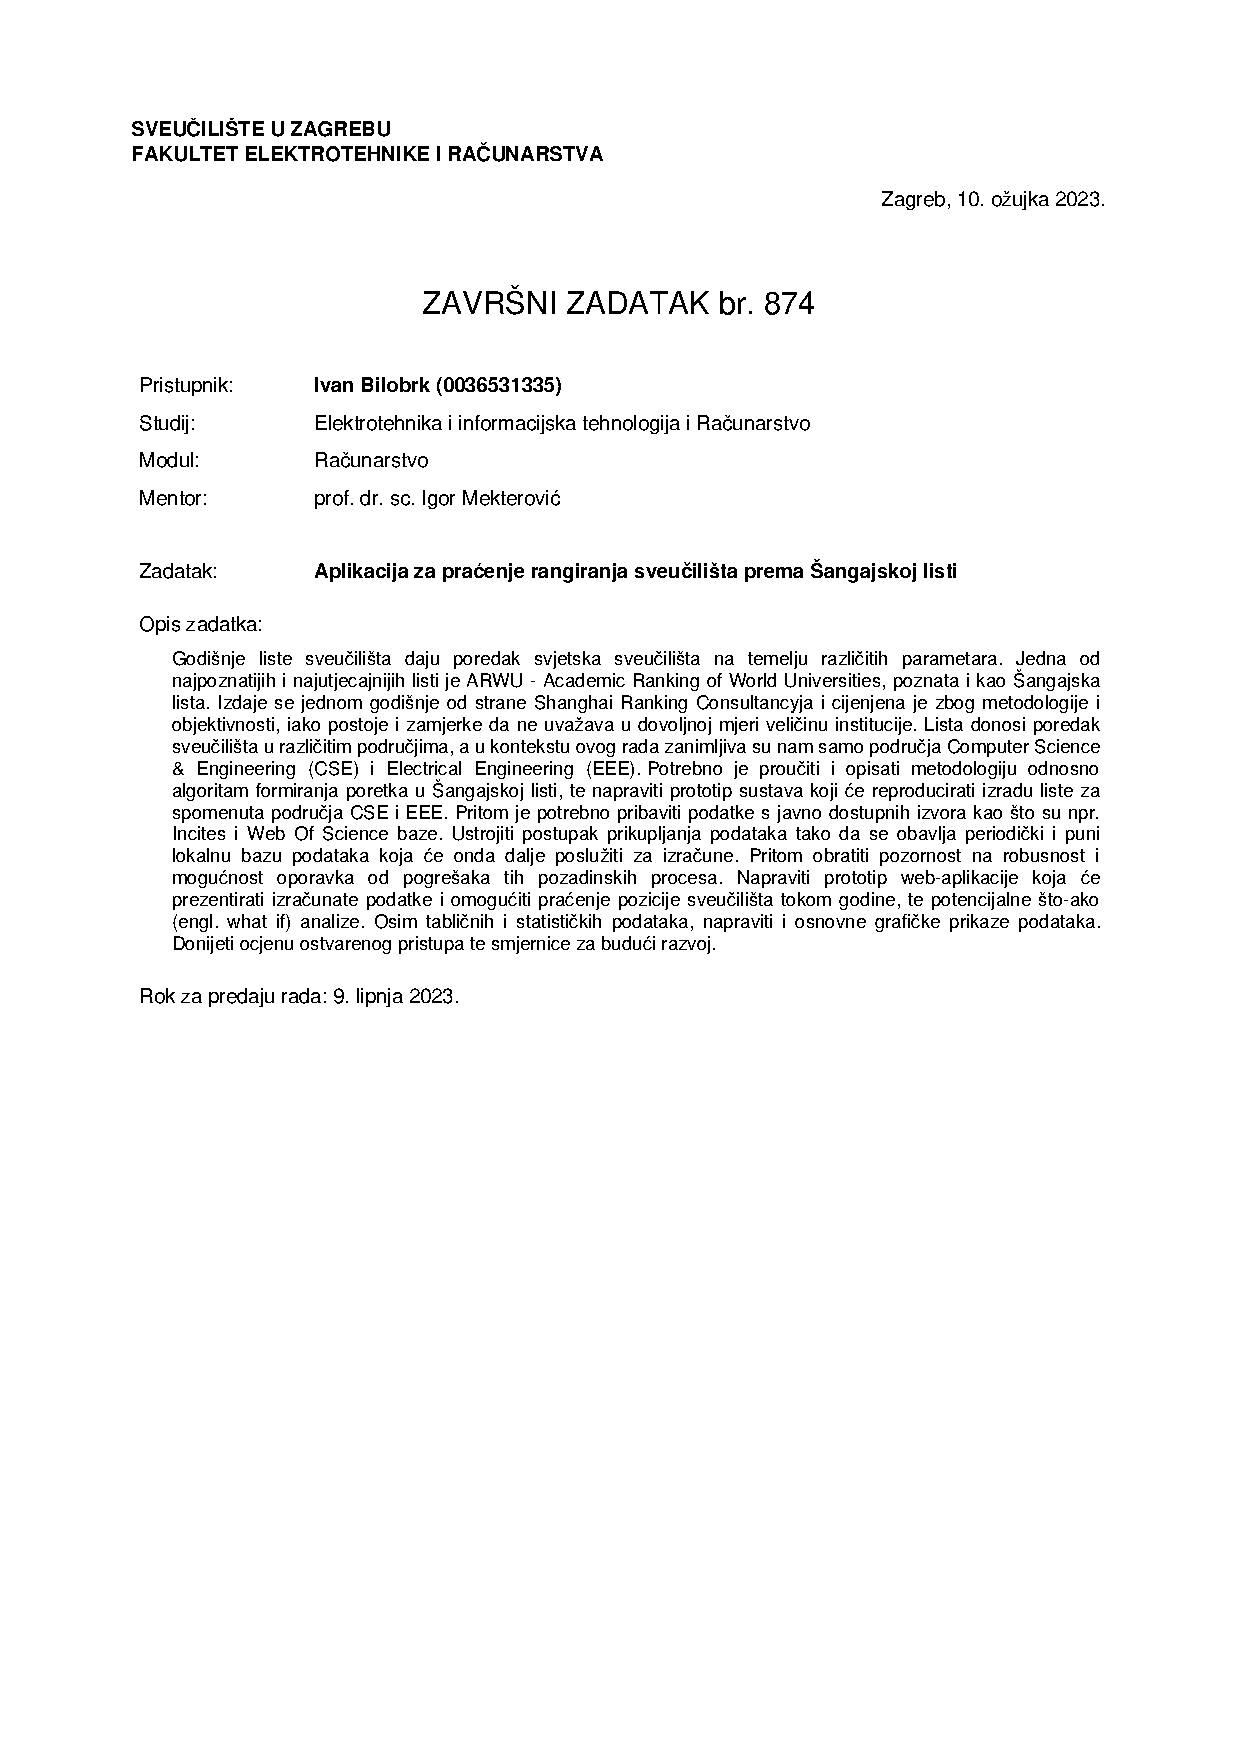
\includepdf[pages=-]{zadatak.pdf}

% Dodavanje zahvale ili prazne stranice. Ako ne želite dodati zahvalu, naredbu ostavite radi prazne stranice.
\zahvala{}

\tableofcontents

\chapter{Uvod}
U svijetu postoji više od 25000 sveučilišta. Svako od njih trudi se imati što bolje predavače, kvalitetniju nastavu, puno znanstvenih radova, sudjelovanja na konferencijama,
objava u časopisima te drugih raznih uspjeha. Sveučilištima je teško uskladiti svoju organizaciju bez neke povratne informacije o svojim uspjesima. Upravo zbog toga napravljene su razne
rang liste koje svakom sveučilištu pridružuju neku numeričku vrijednost te na osnovu nje ih sortiraju. Na ovaj način svako sveučilište dobiva svoju poziciju 
koja može služiti kao mjerilo uspjeha, ukazati na potencijalne probleme na sveučilištu te na taj način omogućiti uvođenje promjena na sveučilištu kako bi 
na sljedećoj rang listi sveučilište bilo na nekoj višoj poziciji.\\ Neke od organizacija koje objavljuju rang liste sveučilišta: Times Higher Education, Round University Ranking,
U.S. News, i Shanghai Ranking. U kontekstu ovog završnog rada, zanima nas način rangiranja Shanghai Ranking sustava. \\ Shanghai Ranking objavljuje jednom godišnje dvije 
rang liste. Prva rangira sveučilišta neovisno o područjima istraživanja i zove se Academic Ranking of World Universities (ARWU). ARWU se objavljuje od 2003. godine i  
temelji se na 6 indikatora uspjeha. Rangira više od 2000 sveučilišta, a samo najboljih 1000 objavi na službenoj stranici. Nama zanimljivija rang lista je Global Ranking of Academic Subjects
(GRAS) koja rangira sveučilišta u nekom području istraživanja. Ovu rang listu Shanghai Ranking objavljuje od 2009. godine. Zadnji ranking, 2022. godine uključivao je više od 1800 sveučilišta 
u više od 96 zemalja u 54 područja istraživanja. Fakultet elektrotehnike i računarstva u Zagrebu (FER) dio je Sveučilišta u Zagrebu te su nam rang liste u području 
računarske znanosti i inženjerstva \engl {Computer Science \& Engineering (CSE)} i elektrotehnike \engl {Electrical \& Electronic Engineering (EEE)} najzanimljivije. Problem tih rang lista 
na Shanghai Ranking stranici je taj što objavljuju samo prvih 500 najboljih sveučilišta u tim područjima što znači da ranking Sveučilišta u Zagrebu ne možemo provjeriti. 
Ovaj završni rad bavi se izradom web aplikacije koja će prikupljati podatke o sveučilištima na isti način kao i Shanghai Ranking, ali uz iznimku da nema ograničenja na 
broj sveučilišta koja se mogu pojaviti na konačnoj rang listi. Na ovaj način Sveučilište u Zagrebu, a i FER moći će pratiti svoj napredak iz godine u godinu te raditi određene 
promjene kako bi im se pozicija na rang listi poboljšala. 

\chapter{Shanghai Ranking metodologija}
Shanghai Ranking Global Ranking of Academic Subjects (GRAS) se objavljuje svake godine i temelji se na podatcima kroz četiri godine.
Ukoliko promatramo ranking za neku godinu $x$,
donja granica godina za podatke je $x-6$, a donja granica je $x-2$. Tako primjerice ukoliko nas zanima ranking za 2022. godinu promatrat ćemo podatke od 2016. do 2020. godine, uključivo.

\section{Izvori za prikupljanje podataka}
Podatke za izračun vrijednosti svih indikatora osim indikatora Award prikupljamo sa baza InCites i Web of Science (WoS). 
Podatke za Award indikator prikupljamo sa raznih stranica ovisno o području koje nas zanima.
Za Computer Science \& Engineering (CSE) to je stranica A.M. Turing Award: \url{https://amturing.acm.org/}, a za Electrical \& Electronic Engineering (EEE) IEEE Awards:
\url{https://corporate-awards.ieee.org/}

\section{Minimalni broj publikacija} Kako bi sveučilište ušlo na ranking za područja Computer Science \& Engineering (CSE) i Electrical \& Electronic Engineering (EEE) mora imati minimalno 150 publikacija koje su vidljive 
na bazama Web of Science (WoS) i InCites.
\\ \section{Preslikavanje područja istraživanja}Kako bi uspješno prikupili podatke sa navedenih baza moramo na tim stranicama odabrati ispravno područje istraživanja jer preslikavanja nisu $1:1$.
\\\\U sljedećim tablicama možemo vidjeti kako izgledaju preslikavanja za područja CSE i EEE.

\begin{table}[htb]
    \caption{Preslikavanje za područje Computer Science \& Engineering (CSE)}
    \label{tbl:konstante}
    \centering
    \begin{tabular}{ll} \hline
    Područje na Shanghai Ranking stranici & Područje na InCites i \\ & Web of Science (WoS) bazama\\ \hline
    Computer Science \& Engineering & Computer Science, Information Systems \\
    Computer Science \& Engineering & Computer Science, Cybernetics \\
    Computer Science \& Engineering & Computer Science, Software Engineering \\
    Computer Science \& Engineering & Computer Science, Artificial Intelligence \\
    Computer Science \& Engineering & Computer Science, Hardware \& Architecture \\
    Computer Science \& Engineering & Computer Science, Theory \& Methods \\
    Computer Science \& Engineering & Computer Science, Interdisciplinary Applications \\
    \end{tabular}
    \end{table}
    \FloatBarrier
    \hfil

\begin{table}[htb]
    \caption{Preslikavanje za područje Electrical \& Electronic Engineering (EEE)}
        \label{tbl:konstante1}
        \centering
        \begin{tabular}{ll} \hline
        Područje na Shanghai Ranking stranici & Područje na InCites i \\ & Web of Science (WoS) bazama\\ \hline
        Electrical \& Electronic Engineering &  Engineering, Electrical \& Electronic\\
        Electrical \& Electronic Engineering &  Imaging Science \& Photographic Technology\\
        \end{tabular}
        \end{table}    
        \FloatBarrier

\section{Indikatori za računanje rankinga}
Global Ranking of Academic Subjects (GRAS) se računa na temelju pet indikatora, a to su: Q1, CNCI, IC, Top i Award.
\\ \textbf{Q1} indikator predstavlja broj publikacija sveučilišta u top $25\%$ časopisa koji su izabrani za neko područje putem ankete ShanghaiRanking’s Academic Excellence Survey
(AES) tijekom relevantnog razdoblja.   
\\ \textbf{CNCI} indikator (Category Normalized Citation Impact) omjer je citiranosti objavljenih radova i prosječnih citiranosti 
radova u istoj kategoriji, iste godine i iste vrste publikacije u časopisu, od strane sveučilišta u određenom području tijekom relevantnog razdoblja.
CNCI vrijednosti manje od 1 znače da je citiranost sveučilišta manja od prosjeka, vrijednost 1 znači da je citiranost prosječna, a vrijednosti veće od
1 znače da je citiranost sveučilišta veća od prosjeka.
\\ \textbf{IC} indikator (International Collaboration) predstavlja koliko međunarodnih suradnja sveučilište u nekom području istraživanja ima.
Točna vrijednost indikatora dobije se kao omjer broja publikacija koje su pronađene u najmanje dvije različite zemlje 
u odnosu na adresu autora prema ukupnom broju publikacija iz odgovarajućeg područja istraživanja za instituciju tijekom relevantnog razdoblja.
\\ \textbf{Top} indikator predstavlja broj radova koje je sveučilište 
objavilo u Top časopisima u nekom području istraživanja tijekom relevantnog razdoblja.
Top časopise biraju profesori sveučilišta isto kao i Q1 časopise kroz anketu ShanghaiRanking’s Academic Excellence Survey (AES). 
Iznimka ovdje je područje Computer Science \& Engineering (CSE) jer se za to područje uzima broj radova predstavljenih na 31 odabranoj konferenciji, 
također kroz ShanghaiRanking’s Academic Excellence Survey (AES).
\\ \textbf{Award} indikator predstavlja broj osoba sveučilišta koje je dobilo značajnu nagradu iz nekog područja istraživanja. Značajne nagrade 
biraju se putem ShanghaiRanking’s Academic Excellence Survey (AES). Značajna nagrada za područje  Computer Science \& Engineering (CSE) je Turingova 
nagrada, a za područje Electrical \& Electronic Engineering (EEE) IEEE Medal of Honor.
Kako bi dobitak nagrade išao u korist sveučilištu, osoba koje je dobila nagradu morala je u trenutku dobitka nagrade raditi puno radno vrijeme na 
tom sveučilištu. Ukoliko je osoba u trenutku dobitka nagrade bila povezana s više sveučilišta ili drugih institucija, svakoj ustanovi se pridjeljuje
recipročan broj broja sveučilišta. Tako na primjer, ako je osoba bila povezana s 3 ustanove, svakoj od njih se pridjeljuje $1/3$, a ako je bila 
povezana samo sa jednom ustanovom pridjeljuje se toj ustanovi $1$. 
Vrijeme dobitka nagrade također igra ulogu jer u obzir dolaze nagrade dodijeljene unazad 4 desetljeća od gornje granice godine za koju promatramo podatke.
Ukoliko nas zanima ranking za 2022. godinu, onda je gornja granica godine za koju promatramo podatke 2020. Svakom desetljeću pridjeljuju se različite težine 
s kojima se onda množi predhodno dobiveni broj. Desetljeću najbližem sadašnjosti pridjeljuje se težina 1, a svim ostalima smanjuje se za 0.25.
Ukupna vrijednost indikatora dobije se zbrajanjem pojedinih vrijednosti za neko sveučilište u nekom području.

\begin{table}[htb]
    \caption{Primjer težina za indikator Award za ranking 2022. godine}
        \label{tbl:konstante2}
        \centering
        \begin{tabular}{cccc} \hline
        2011.-2020. & 2001.-2010. & 1991.-2000. & 1981.-1990.\\ \hline
        1&0.75&0.5&0.25\\
        \end{tabular}
        \end{table}    
        \FloatBarrier
\newpage
\section{Računanje ukupnog rezultata sveučilišta}
Jednom kada imamo sve indikatore za neko sveučilište ukupna brojčana vrijednost prema kojoj ćemo rangirati sveučilišta izračuna 
se na sljedeći način:
\\Svaki od indikatora osim CNCI podijelimo sa najvećom vrijednosti indikatora od svih sveučilišta, iz tog broja izvadimo 
drugi korijen te dobiveni broj pomožimo sa težinom tog indikatora.
Na kraju dobivene vrijednosti sumiramo.
\\
\\ Izračun vrijednosti za neki indikator: 
\begin{align}
    \sqrt[\leftroot{-2}]{\frac{vrijednost \; indikatora}{max(indikator)}} \; * tezina(indikator) \label{eq:a}
\end{align}
\\ Indikator CNCI je poseban te se njegova vrijednost računa na sljedeći način: \\ 
\begin{align}
    \sqrt[\leftroot{-2}]{\frac{vrijednost \; CNCI \; indikatora}{min(2*average(CNCI), max(CNCI))}} \; * tezina(CNCI) \label{eq:b}
    \end{align}
\\ Ukoliko je vrijednost CNCI indikatora veća od vrijednosti brojnika u izrazu \ref{eq:b} onda se sveučilištu automatski pridjeljuje vrijednost 100.

\begin{table}[htb]
    \caption{Težine s kojima množimo indikatore}
        \label{tbl:konstante3}
        \centering
        \begin{tabular}{ccccc} \hline
        Q1 & CNCI & IC & Top & Award \\ \hline
        100&100&20&100&100\\
        \end{tabular}
        \end{table}    
        \FloatBarrier


\subsection{Primjer izračuna vrijednosti za ranking}
Promatramo izračun vrijednosti za sveučilište University of California, Berkeley koje je 2022. godine bilo prvo na rankingu u području 
Electrical \& Electronic Engineering (EEE).
\\
\\ \underline{Vrijednost Q1:} 
\\ Pretraživanjem InCites baze vidimo da navedeno sveučilište ima vrijednost indikatora Q1 603. Najveća vrijednost Q1 indikatora u tom razdoblju iznosi 3285.
Vrijednost koja se veže za Q1 indikator iznosi;  \; $\sqrt[\leftroot{-2}]{\frac{603}{3285}} \; * 100 = 42.8$
\\
\\ \underline{Vrijednost CNCI:} 
\\ Pretraživanjem InCites baze vidimo da navedeno sveučilište ima vrijednost indikatora CNCI 1.71. Najveća vrijednost CNCI indikatora u tom razdoblju iznosi 4.13.
Kako je riječ o indikatoru CNCI u obzir još moramo uzeti i dvostruku prosječnu vrijednost svih CNCI vrijednosti, a to je 2.27.
Vrijednost koja se veže za Q1 indikator iznosi: \; \\ $\sqrt[\leftroot{-2}]{\frac{1.71}{min(2.27, 4.13)}} \; * 100 = 86.8$
\\
\\ \underline{Vrijednost IC:} 
\\ Pretraživanjem InCites baze vidimo da navedeno sveučilište ima vrijednost indikatora IC 57.18. Najveća vrijednost IC indikatora u tom razdoblju iznosi 97.15.
Vrijednost koja se veže za IC indikator iznosi: \; \\ $\sqrt[\leftroot{-2}]{\frac{57.18}{97.15}} \; * 20 = 15.3$
\\
\\ \underline{Vrijednost Top:} 
\\ Pretraživanjem InCites baze vidimo da navedeno sveučilište ima vrijednost indikatora Top 25. Najveća vrijednost Top indikatora u tom razdoblju iznosi 25.
Vrijednost koja se veže za Top indikator iznosi: \; \\ $\sqrt[\leftroot{-2}]{\frac{25}{25}} \; * 100 = 100$
\\
\\ \underline{Vrijednost Award:} 
\\ Pretraživanjem stranice IEEE Awards vidimo da je navedeno sveučilište osvojilo nagradu IEEE Medal of Honor sljedećih godina: 1985., 1995., 1998., 2020. Kako je 
svake godine nagradu osvojila uvijek jedna osoba koja nije bila vezana za nijednu drugu ustanovu, vrijednost 
indikatora Award je $1*0.25+1*0.5+1*0.5+1*1 = 2.25$ (u obzir uzimamo težine koje se vežu za godinu osvajanja nagrade). Najveća vrijednost 
indikatora Award u tom razdoblju iznosi 3. Vrijednost koja se veže za Award indikator iznosi: \; \\ $\sqrt[\leftroot{-2}]{\frac{2.25}{3}} \; * 100 = 86.6$
\\Ukupan rezultat sveučilišta University of California, Berkeley 2022. godine iznosi: $42.8+86.8+15.3+100+86.6 = 331.5$ 






        
        


\chapter{Zaključak}
Zaključak.

\bibliography{literatura}
\bibliographystyle{fer}

\begin{sazetak}
Sažetak na hrvatskom jeziku.

\kljucnerijeci{Ključne riječi, odvojene zarezima.}
\end{sazetak}

% TODO: Navedite naslov na engleskom jeziku.
\engtitle{Title}
\begin{abstract}
Abstract.

\keywords{Keywords.}
\end{abstract}

\end{document}
